\documentclass[twoside]{book}

% Packages required by doxygen
\usepackage{fixltx2e}
\usepackage{calc}
\usepackage{doxygen}
\usepackage[export]{adjustbox} % also loads graphicx
\usepackage{graphicx}
\usepackage[utf8]{inputenc}
\usepackage{makeidx}
\usepackage{multicol}
\usepackage{multirow}
\PassOptionsToPackage{warn}{textcomp}
\usepackage{textcomp}
\usepackage[nointegrals]{wasysym}
\usepackage[table]{xcolor}

% Font selection
\usepackage[T1]{fontenc}
\usepackage[scaled=.90]{helvet}
\usepackage{courier}
\usepackage{amssymb}
\usepackage{sectsty}
\renewcommand{\familydefault}{\sfdefault}
\allsectionsfont{%
  \fontseries{bc}\selectfont%
  \color{darkgray}%
}
\renewcommand{\DoxyLabelFont}{%
  \fontseries{bc}\selectfont%
  \color{darkgray}%
}
\newcommand{\+}{\discretionary{\mbox{\scriptsize$\hookleftarrow$}}{}{}}

% Page & text layout
\usepackage{geometry}
\geometry{%
  a4paper,%
  top=2.5cm,%
  bottom=2.5cm,%
  left=2.5cm,%
  right=2.5cm%
}
\tolerance=750
\hfuzz=15pt
\hbadness=750
\setlength{\emergencystretch}{15pt}
\setlength{\parindent}{0cm}
\setlength{\parskip}{3ex plus 2ex minus 2ex}
\makeatletter
\renewcommand{\paragraph}{%
  \@startsection{paragraph}{4}{0ex}{-1.0ex}{1.0ex}{%
    \normalfont\normalsize\bfseries\SS@parafont%
  }%
}
\renewcommand{\subparagraph}{%
  \@startsection{subparagraph}{5}{0ex}{-1.0ex}{1.0ex}{%
    \normalfont\normalsize\bfseries\SS@subparafont%
  }%
}
\makeatother

% Headers & footers
\usepackage{fancyhdr}
\pagestyle{fancyplain}
\fancyhead[LE]{\fancyplain{}{\bfseries\thepage}}
\fancyhead[CE]{\fancyplain{}{}}
\fancyhead[RE]{\fancyplain{}{\bfseries\leftmark}}
\fancyhead[LO]{\fancyplain{}{\bfseries\rightmark}}
\fancyhead[CO]{\fancyplain{}{}}
\fancyhead[RO]{\fancyplain{}{\bfseries\thepage}}
\fancyfoot[LE]{\fancyplain{}{}}
\fancyfoot[CE]{\fancyplain{}{}}
\fancyfoot[RE]{\fancyplain{}{\bfseries\scriptsize Generated by Doxygen }}
\fancyfoot[LO]{\fancyplain{}{\bfseries\scriptsize Generated by Doxygen }}
\fancyfoot[CO]{\fancyplain{}{}}
\fancyfoot[RO]{\fancyplain{}{}}
\renewcommand{\footrulewidth}{0.4pt}
\renewcommand{\chaptermark}[1]{%
  \markboth{#1}{}%
}
\renewcommand{\sectionmark}[1]{%
  \markright{\thesection\ #1}%
}

% Indices & bibliography
\usepackage{natbib}
\usepackage[titles]{tocloft}
\setcounter{tocdepth}{3}
\setcounter{secnumdepth}{5}
\makeindex

% Hyperlinks (required, but should be loaded last)
\usepackage{ifpdf}
\ifpdf
  \usepackage[pdftex,pagebackref=true]{hyperref}
\else
  \usepackage[ps2pdf,pagebackref=true]{hyperref}
\fi
\hypersetup{%
  colorlinks=true,%
  linkcolor=blue,%
  citecolor=blue,%
  unicode%
}

% Custom commands
\newcommand{\clearemptydoublepage}{%
  \newpage{\pagestyle{empty}\cleardoublepage}%
}

\usepackage{caption}
\captionsetup{labelsep=space,justification=centering,font={bf},singlelinecheck=off,skip=4pt,position=top}

%===== C O N T E N T S =====

\begin{document}

% Titlepage & ToC
\hypersetup{pageanchor=false,
             bookmarksnumbered=true,
             pdfencoding=unicode
            }
\pagenumbering{alph}
\begin{titlepage}
\vspace*{7cm}
\begin{center}%
{\Large Heisprosjekt }\\
\vspace*{1cm}
{\large Generated by Doxygen 1.8.13}\\
\end{center}
\end{titlepage}
\clearemptydoublepage
\pagenumbering{roman}
\tableofcontents
\clearemptydoublepage
\pagenumbering{arabic}
\hypersetup{pageanchor=true}

%--- Begin generated contents ---
\chapter{File Index}
\section{File List}
Here is a list of all documented files with brief descriptions\+:\begin{DoxyCompactList}
\item\contentsline{section}{source/\hyperlink{hardware_8h}{hardware.\+h} \\*Driver for the elevator hardware }{\pageref{hardware_8h}}{}
\item\contentsline{section}{source/{\bfseries main.\+c} }{\pageref{main_8c}}{}
\item\contentsline{section}{source/{\bfseries queue.\+c} }{\pageref{queue_8c}}{}
\item\contentsline{section}{source/\hyperlink{queue_8h}{queue.\+h} \\*Implements queue system for orders }{\pageref{queue_8h}}{}
\item\contentsline{section}{source/{\bfseries timer.\+c} }{\pageref{timer_8c}}{}
\item\contentsline{section}{source/\hyperlink{timer_8h}{timer.\+h} \\*Timer functionality }{\pageref{timer_8h}}{}
\item\contentsline{section}{source/{\bfseries utilities.\+c} }{\pageref{utilities_8c}}{}
\item\contentsline{section}{source/\hyperlink{utilities_8h}{utilities.\+h} \\*Various utilities to simplify interaction with hardware }{\pageref{utilities_8h}}{}
\end{DoxyCompactList}

\chapter{File Documentation}
\hypertarget{hardware_8h}{}\section{source/hardware.h File Reference}
\label{hardware_8h}\index{source/hardware.\+h@{source/hardware.\+h}}


Driver for the elevator hardware.  


This graph shows which files directly or indirectly include this file\+:
\nopagebreak
\begin{figure}[H]
\begin{center}
\leavevmode
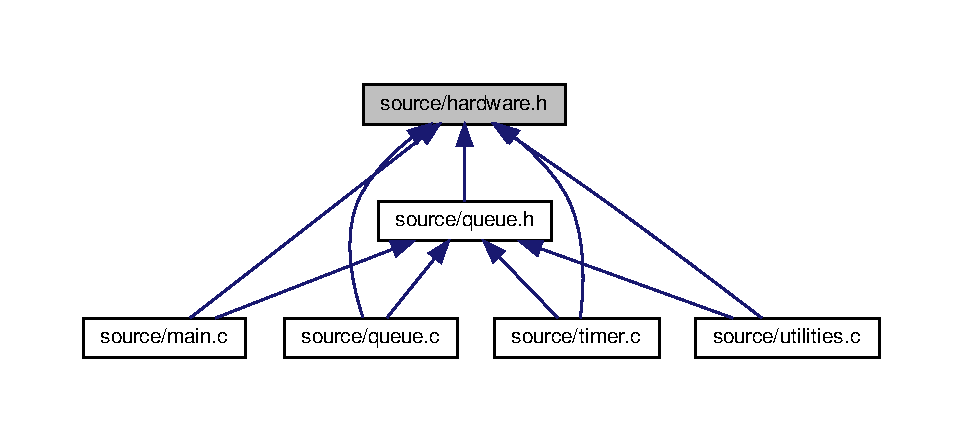
\includegraphics[width=350pt]{hardware_8h__dep__incl}
\end{center}
\end{figure}
\subsection*{Macros}
\begin{DoxyCompactItemize}
\item 
\mbox{\Hypertarget{hardware_8h_ae9e42615eade15633bd8c03b7a271a00}\label{hardware_8h_ae9e42615eade15633bd8c03b7a271a00}} 
\#define {\bfseries H\+A\+R\+D\+W\+A\+R\+E\+\_\+\+N\+U\+M\+B\+E\+R\+\_\+\+O\+F\+\_\+\+F\+L\+O\+O\+RS}~4
\end{DoxyCompactItemize}
\subsection*{Enumerations}
\begin{DoxyCompactItemize}
\item 
\mbox{\Hypertarget{hardware_8h_a2167c399a24df296afc432bcb88228af}\label{hardware_8h_a2167c399a24df296afc432bcb88228af}} 
enum \hyperlink{hardware_8h_a2167c399a24df296afc432bcb88228af}{Hardware\+Movement} \{ {\bfseries H\+A\+R\+D\+W\+A\+R\+E\+\_\+\+M\+O\+V\+E\+M\+E\+N\+T\+\_\+\+UP}, 
{\bfseries H\+A\+R\+D\+W\+A\+R\+E\+\_\+\+M\+O\+V\+E\+M\+E\+N\+T\+\_\+\+S\+T\+OP}, 
{\bfseries H\+A\+R\+D\+W\+A\+R\+E\+\_\+\+M\+O\+V\+E\+M\+E\+N\+T\+\_\+\+D\+O\+WN}
 \}\begin{DoxyCompactList}\small\item\em Movement type used in {\ttfamily hardware\+\_\+command\+\_\+movement}. \end{DoxyCompactList}
\item 
\mbox{\Hypertarget{hardware_8h_a796a8de8ce0ae769d7dbd3327a7bdbe7}\label{hardware_8h_a796a8de8ce0ae769d7dbd3327a7bdbe7}} 
enum \hyperlink{hardware_8h_a796a8de8ce0ae769d7dbd3327a7bdbe7}{Hardware\+Order} \{ {\bfseries H\+A\+R\+D\+W\+A\+R\+E\+\_\+\+O\+R\+D\+E\+R\+\_\+\+UP}, 
{\bfseries H\+A\+R\+D\+W\+A\+R\+E\+\_\+\+O\+R\+D\+E\+R\+\_\+\+I\+N\+S\+I\+DE}, 
{\bfseries H\+A\+R\+D\+W\+A\+R\+E\+\_\+\+O\+R\+D\+E\+R\+\_\+\+D\+O\+WN}
 \}\begin{DoxyCompactList}\small\item\em Order type used in {\ttfamily hardware\+\_\+read\+\_\+order} and in {\ttfamily hardware\+\_\+command\+\_\+order\+\_\+light}. \end{DoxyCompactList}
\end{DoxyCompactItemize}
\subsection*{Functions}
\begin{DoxyCompactItemize}
\item 
int \hyperlink{hardware_8h_a054b8fb8768311d46be58d6a4890d771}{hardware\+\_\+init} ()
\begin{DoxyCompactList}\small\item\em Initializes the elevator control hardware. Must be called once before other calls to the elevator hardware driver. \end{DoxyCompactList}\item 
void \hyperlink{hardware_8h_a01de081ef0510a111053c18cd31afa27}{hardware\+\_\+command\+\_\+movement} (\hyperlink{hardware_8h_a2167c399a24df296afc432bcb88228af}{Hardware\+Movement} movement)
\begin{DoxyCompactList}\small\item\em Commands the elevator to either move up or down, or commands it to halt. \end{DoxyCompactList}\item 
int \hyperlink{hardware_8h_a4a77b27c86675c00b513db3445966804}{hardware\+\_\+read\+\_\+stop\+\_\+signal} ()
\begin{DoxyCompactList}\small\item\em Polls the hardware for the current stop signal. \end{DoxyCompactList}\item 
int \hyperlink{hardware_8h_a459fe57a3ee4bc2a28e8a15b2ab14c2d}{hardware\+\_\+read\+\_\+obstruction\+\_\+signal} ()
\begin{DoxyCompactList}\small\item\em Polls the hardware for the current obstruction signal. \end{DoxyCompactList}\item 
int \hyperlink{hardware_8h_ab048489e6302bb5604aad753f2d7d501}{hardware\+\_\+read\+\_\+floor\+\_\+sensor} (int floor)
\begin{DoxyCompactList}\small\item\em Polls the floor sensor for the given {\ttfamily floor}. \end{DoxyCompactList}\item 
int \hyperlink{hardware_8h_a87917f3aa093fb46ca821a400d011ee8}{hardware\+\_\+read\+\_\+order} (int floor, \hyperlink{hardware_8h_a796a8de8ce0ae769d7dbd3327a7bdbe7}{Hardware\+Order} order\+\_\+type)
\begin{DoxyCompactList}\small\item\em Polls the hardware for the status of orders from floor {\ttfamily floor} of type {\ttfamily order\+\_\+type}. \end{DoxyCompactList}\item 
void \hyperlink{hardware_8h_a80d99ddaa8e7b58c9a88b60ea553c1b6}{hardware\+\_\+command\+\_\+door\+\_\+open} (int door\+\_\+open)
\begin{DoxyCompactList}\small\item\em Commands the hardware to open-\/ or close the elevator door. \end{DoxyCompactList}\item 
void \hyperlink{hardware_8h_a407a6ec035ba357de6aa0fbe55501d1e}{hardware\+\_\+command\+\_\+floor\+\_\+indicator\+\_\+on} (int floor)
\begin{DoxyCompactList}\small\item\em Commands the hardware to turn on the floor indicator for {\ttfamily floor}. All indicators all mutually exclusive; other indicator lights will turn off. \end{DoxyCompactList}\item 
void \hyperlink{hardware_8h_aa75b3ac17f72b25946414f48d0063a10}{hardware\+\_\+command\+\_\+stop\+\_\+light} (int on)
\begin{DoxyCompactList}\small\item\em Sets the light in the panel stop button. \end{DoxyCompactList}\item 
void \hyperlink{hardware_8h_aa9b33faa52f0ec5b614d3e7dc05be140}{hardware\+\_\+command\+\_\+order\+\_\+light} (int floor, \hyperlink{hardware_8h_a796a8de8ce0ae769d7dbd3327a7bdbe7}{Hardware\+Order} order\+\_\+type, int on)
\begin{DoxyCompactList}\small\item\em Sets the light in a button corresponding to an order of type {\ttfamily order\+\_\+type}, at floor {\ttfamily floor}. \end{DoxyCompactList}\end{DoxyCompactItemize}


\subsection{Detailed Description}
Driver for the elevator hardware. 

Neatly wraps up Martin Korsgaard\textquotesingle{}s spaghetti from 2006 ;)

Kolbjørn Austreng 

\subsection{Function Documentation}
\mbox{\Hypertarget{hardware_8h_a80d99ddaa8e7b58c9a88b60ea553c1b6}\label{hardware_8h_a80d99ddaa8e7b58c9a88b60ea553c1b6}} 
\index{hardware.\+h@{hardware.\+h}!hardware\+\_\+command\+\_\+door\+\_\+open@{hardware\+\_\+command\+\_\+door\+\_\+open}}
\index{hardware\+\_\+command\+\_\+door\+\_\+open@{hardware\+\_\+command\+\_\+door\+\_\+open}!hardware.\+h@{hardware.\+h}}
\subsubsection{\texorpdfstring{hardware\+\_\+command\+\_\+door\+\_\+open()}{hardware\_command\_door\_open()}}
{\footnotesize\ttfamily void hardware\+\_\+command\+\_\+door\+\_\+open (\begin{DoxyParamCaption}\item[{int}]{door\+\_\+open }\end{DoxyParamCaption})}



Commands the hardware to open-\/ or close the elevator door. 


\begin{DoxyParams}{Parameters}
{\em door\+\_\+open} & A truthy value (non-\/zero) to open the door; 0 to close. \\
\hline
\end{DoxyParams}
\mbox{\Hypertarget{hardware_8h_a407a6ec035ba357de6aa0fbe55501d1e}\label{hardware_8h_a407a6ec035ba357de6aa0fbe55501d1e}} 
\index{hardware.\+h@{hardware.\+h}!hardware\+\_\+command\+\_\+floor\+\_\+indicator\+\_\+on@{hardware\+\_\+command\+\_\+floor\+\_\+indicator\+\_\+on}}
\index{hardware\+\_\+command\+\_\+floor\+\_\+indicator\+\_\+on@{hardware\+\_\+command\+\_\+floor\+\_\+indicator\+\_\+on}!hardware.\+h@{hardware.\+h}}
\subsubsection{\texorpdfstring{hardware\+\_\+command\+\_\+floor\+\_\+indicator\+\_\+on()}{hardware\_command\_floor\_indicator\_on()}}
{\footnotesize\ttfamily void hardware\+\_\+command\+\_\+floor\+\_\+indicator\+\_\+on (\begin{DoxyParamCaption}\item[{int}]{floor }\end{DoxyParamCaption})}



Commands the hardware to turn on the floor indicator for {\ttfamily floor}. All indicators all mutually exclusive; other indicator lights will turn off. 


\begin{DoxyParams}{Parameters}
{\em floor} & Floor to turn on the indicator for.\\
\hline
\end{DoxyParams}
\begin{DoxyWarning}{Warning}
Owing to peculiarities in the hardware construction, there will always be one indicator active. 
\end{DoxyWarning}
\mbox{\Hypertarget{hardware_8h_a01de081ef0510a111053c18cd31afa27}\label{hardware_8h_a01de081ef0510a111053c18cd31afa27}} 
\index{hardware.\+h@{hardware.\+h}!hardware\+\_\+command\+\_\+movement@{hardware\+\_\+command\+\_\+movement}}
\index{hardware\+\_\+command\+\_\+movement@{hardware\+\_\+command\+\_\+movement}!hardware.\+h@{hardware.\+h}}
\subsubsection{\texorpdfstring{hardware\+\_\+command\+\_\+movement()}{hardware\_command\_movement()}}
{\footnotesize\ttfamily void hardware\+\_\+command\+\_\+movement (\begin{DoxyParamCaption}\item[{\hyperlink{hardware_8h_a2167c399a24df296afc432bcb88228af}{Hardware\+Movement}}]{movement }\end{DoxyParamCaption})}



Commands the elevator to either move up or down, or commands it to halt. 


\begin{DoxyParams}{Parameters}
{\em movement} & Commanded movement. \\
\hline
\end{DoxyParams}
\mbox{\Hypertarget{hardware_8h_aa9b33faa52f0ec5b614d3e7dc05be140}\label{hardware_8h_aa9b33faa52f0ec5b614d3e7dc05be140}} 
\index{hardware.\+h@{hardware.\+h}!hardware\+\_\+command\+\_\+order\+\_\+light@{hardware\+\_\+command\+\_\+order\+\_\+light}}
\index{hardware\+\_\+command\+\_\+order\+\_\+light@{hardware\+\_\+command\+\_\+order\+\_\+light}!hardware.\+h@{hardware.\+h}}
\subsubsection{\texorpdfstring{hardware\+\_\+command\+\_\+order\+\_\+light()}{hardware\_command\_order\_light()}}
{\footnotesize\ttfamily void hardware\+\_\+command\+\_\+order\+\_\+light (\begin{DoxyParamCaption}\item[{int}]{floor,  }\item[{\hyperlink{hardware_8h_a796a8de8ce0ae769d7dbd3327a7bdbe7}{Hardware\+Order}}]{order\+\_\+type,  }\item[{int}]{on }\end{DoxyParamCaption})}



Sets the light in a button corresponding to an order of type {\ttfamily order\+\_\+type}, at floor {\ttfamily floor}. 


\begin{DoxyParams}{Parameters}
{\em floor} & The floor of the order indicator. \\
\hline
{\em order\+\_\+type} & The type of order. \\
\hline
{\em on} & A truthy value (non-\/zero) to turn the light on; 0 to turn it off. \\
\hline
\end{DoxyParams}
\mbox{\Hypertarget{hardware_8h_aa75b3ac17f72b25946414f48d0063a10}\label{hardware_8h_aa75b3ac17f72b25946414f48d0063a10}} 
\index{hardware.\+h@{hardware.\+h}!hardware\+\_\+command\+\_\+stop\+\_\+light@{hardware\+\_\+command\+\_\+stop\+\_\+light}}
\index{hardware\+\_\+command\+\_\+stop\+\_\+light@{hardware\+\_\+command\+\_\+stop\+\_\+light}!hardware.\+h@{hardware.\+h}}
\subsubsection{\texorpdfstring{hardware\+\_\+command\+\_\+stop\+\_\+light()}{hardware\_command\_stop\_light()}}
{\footnotesize\ttfamily void hardware\+\_\+command\+\_\+stop\+\_\+light (\begin{DoxyParamCaption}\item[{int}]{on }\end{DoxyParamCaption})}



Sets the light in the panel stop button. 


\begin{DoxyParams}{Parameters}
{\em on} & A truthy value (non-\/zero) to turn the light on; 0 to turn it off. \\
\hline
\end{DoxyParams}
\mbox{\Hypertarget{hardware_8h_a054b8fb8768311d46be58d6a4890d771}\label{hardware_8h_a054b8fb8768311d46be58d6a4890d771}} 
\index{hardware.\+h@{hardware.\+h}!hardware\+\_\+init@{hardware\+\_\+init}}
\index{hardware\+\_\+init@{hardware\+\_\+init}!hardware.\+h@{hardware.\+h}}
\subsubsection{\texorpdfstring{hardware\+\_\+init()}{hardware\_init()}}
{\footnotesize\ttfamily int hardware\+\_\+init (\begin{DoxyParamCaption}{ }\end{DoxyParamCaption})}



Initializes the elevator control hardware. Must be called once before other calls to the elevator hardware driver. 

\begin{DoxyReturn}{Returns}
0 on success. Non-\/zero for failure. 
\end{DoxyReturn}
\mbox{\Hypertarget{hardware_8h_ab048489e6302bb5604aad753f2d7d501}\label{hardware_8h_ab048489e6302bb5604aad753f2d7d501}} 
\index{hardware.\+h@{hardware.\+h}!hardware\+\_\+read\+\_\+floor\+\_\+sensor@{hardware\+\_\+read\+\_\+floor\+\_\+sensor}}
\index{hardware\+\_\+read\+\_\+floor\+\_\+sensor@{hardware\+\_\+read\+\_\+floor\+\_\+sensor}!hardware.\+h@{hardware.\+h}}
\subsubsection{\texorpdfstring{hardware\+\_\+read\+\_\+floor\+\_\+sensor()}{hardware\_read\_floor\_sensor()}}
{\footnotesize\ttfamily int hardware\+\_\+read\+\_\+floor\+\_\+sensor (\begin{DoxyParamCaption}\item[{int}]{floor }\end{DoxyParamCaption})}



Polls the floor sensor for the given {\ttfamily floor}. 


\begin{DoxyParams}{Parameters}
{\em floor} & Inquired floor.\\
\hline
\end{DoxyParams}
\begin{DoxyReturn}{Returns}
1 if the elevator is at {\ttfamily floor}, otherwise 0; 
\end{DoxyReturn}
\mbox{\Hypertarget{hardware_8h_a459fe57a3ee4bc2a28e8a15b2ab14c2d}\label{hardware_8h_a459fe57a3ee4bc2a28e8a15b2ab14c2d}} 
\index{hardware.\+h@{hardware.\+h}!hardware\+\_\+read\+\_\+obstruction\+\_\+signal@{hardware\+\_\+read\+\_\+obstruction\+\_\+signal}}
\index{hardware\+\_\+read\+\_\+obstruction\+\_\+signal@{hardware\+\_\+read\+\_\+obstruction\+\_\+signal}!hardware.\+h@{hardware.\+h}}
\subsubsection{\texorpdfstring{hardware\+\_\+read\+\_\+obstruction\+\_\+signal()}{hardware\_read\_obstruction\_signal()}}
{\footnotesize\ttfamily int hardware\+\_\+read\+\_\+obstruction\+\_\+signal (\begin{DoxyParamCaption}{ }\end{DoxyParamCaption})}



Polls the hardware for the current obstruction signal. 

\begin{DoxyReturn}{Returns}
1 if the obstruction signal is high; 0 if it is low. 
\end{DoxyReturn}
\mbox{\Hypertarget{hardware_8h_a87917f3aa093fb46ca821a400d011ee8}\label{hardware_8h_a87917f3aa093fb46ca821a400d011ee8}} 
\index{hardware.\+h@{hardware.\+h}!hardware\+\_\+read\+\_\+order@{hardware\+\_\+read\+\_\+order}}
\index{hardware\+\_\+read\+\_\+order@{hardware\+\_\+read\+\_\+order}!hardware.\+h@{hardware.\+h}}
\subsubsection{\texorpdfstring{hardware\+\_\+read\+\_\+order()}{hardware\_read\_order()}}
{\footnotesize\ttfamily int hardware\+\_\+read\+\_\+order (\begin{DoxyParamCaption}\item[{int}]{floor,  }\item[{\hyperlink{hardware_8h_a796a8de8ce0ae769d7dbd3327a7bdbe7}{Hardware\+Order}}]{order\+\_\+type }\end{DoxyParamCaption})}



Polls the hardware for the status of orders from floor {\ttfamily floor} of type {\ttfamily order\+\_\+type}. 


\begin{DoxyParams}{Parameters}
{\em floor} & Inquired floor. \\
\hline
{\em order\+\_\+type} & \\
\hline
\end{DoxyParams}
\begin{DoxyReturn}{Returns}
1 if the combination of {\ttfamily floor} and {\ttfamily order\+\_\+type} is being requested, otherwise 0. 
\end{DoxyReturn}
\mbox{\Hypertarget{hardware_8h_a4a77b27c86675c00b513db3445966804}\label{hardware_8h_a4a77b27c86675c00b513db3445966804}} 
\index{hardware.\+h@{hardware.\+h}!hardware\+\_\+read\+\_\+stop\+\_\+signal@{hardware\+\_\+read\+\_\+stop\+\_\+signal}}
\index{hardware\+\_\+read\+\_\+stop\+\_\+signal@{hardware\+\_\+read\+\_\+stop\+\_\+signal}!hardware.\+h@{hardware.\+h}}
\subsubsection{\texorpdfstring{hardware\+\_\+read\+\_\+stop\+\_\+signal()}{hardware\_read\_stop\_signal()}}
{\footnotesize\ttfamily int hardware\+\_\+read\+\_\+stop\+\_\+signal (\begin{DoxyParamCaption}{ }\end{DoxyParamCaption})}



Polls the hardware for the current stop signal. 

\begin{DoxyReturn}{Returns}
1 if the stop signal is high; 0 if it is low. 
\end{DoxyReturn}

\hypertarget{queue_8h}{}\section{source/queue.h File Reference}
\label{queue_8h}\index{source/queue.\+h@{source/queue.\+h}}


Implements queue system for orders.  


{\ttfamily \#include $<$stdbool.\+h$>$}\newline
{\ttfamily \#include \char`\"{}hardware.\+h\char`\"{}}\newline
Include dependency graph for queue.\+h\+:
\nopagebreak
\begin{figure}[H]
\begin{center}
\leavevmode
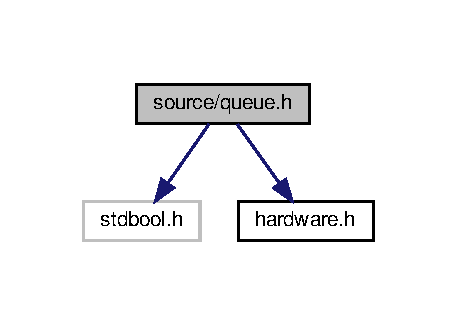
\includegraphics[width=220pt]{queue_8h__incl}
\end{center}
\end{figure}
This graph shows which files directly or indirectly include this file\+:
\nopagebreak
\begin{figure}[H]
\begin{center}
\leavevmode
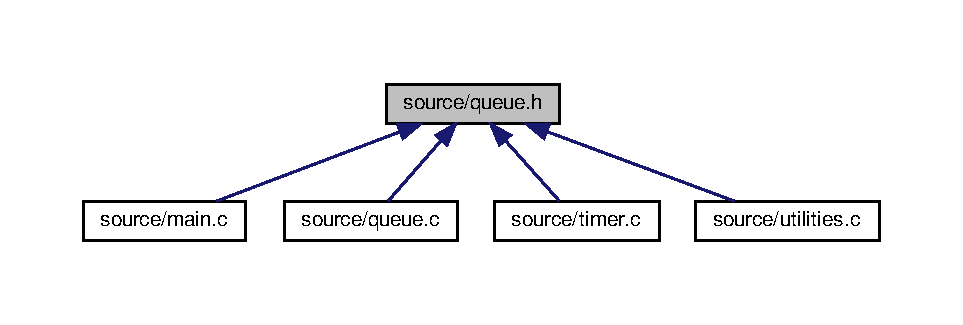
\includegraphics[width=350pt]{queue_8h__dep__incl}
\end{center}
\end{figure}
\subsection*{Functions}
\begin{DoxyCompactItemize}
\item 
int \hyperlink{queue_8h_add3ac34d70f5081d02bf2b05d19fb70f}{order\+\_\+to\+\_\+int\+\_\+encoding} (int floor, \hyperlink{hardware_8h_a796a8de8ce0ae769d7dbd3327a7bdbe7}{Hardware\+Order} type)
\begin{DoxyCompactList}\small\item\em Encodes order to corresponding int. \end{DoxyCompactList}\item 
void \hyperlink{queue_8h_a83a8924c00e2569b5bc6dea377e1fb87}{add\+\_\+order} (int floor, \hyperlink{hardware_8h_a796a8de8ce0ae769d7dbd3327a7bdbe7}{Hardware\+Order} type, int($\ast$orders)\mbox{[}10\mbox{]}, int array\+\_\+size)
\begin{DoxyCompactList}\small\item\em Adds an order to the queue, {\ttfamily orders}. \end{DoxyCompactList}\item 
void \hyperlink{queue_8h_a02cca89cc902f09b6e7122879992155d}{del\+\_\+all\+\_\+orders\+\_\+on\+\_\+floor} (int floor, int($\ast$orders)\mbox{[}10\mbox{]}, int array\+\_\+size)
\begin{DoxyCompactList}\small\item\em Deletes all orders on specified {\ttfamily floor} from the queue, {\ttfamily orders}, then restacks the queue. \end{DoxyCompactList}\item 
void \hyperlink{queue_8h_a4b29ca8e212d3b7668fc8e0b3e142b77}{del\+\_\+all\+\_\+orders} (int($\ast$orders)\mbox{[}10\mbox{]}, int array\+\_\+size)
\begin{DoxyCompactList}\small\item\em Deletes all orders in queue, {\ttfamily orders}. \end{DoxyCompactList}\item 
bool \hyperlink{queue_8h_a51cac483ef97f6cd2b7e87b2567a0f75}{check\+\_\+queue\+\_\+for\+\_\+order} (int floor, \hyperlink{hardware_8h_a796a8de8ce0ae769d7dbd3327a7bdbe7}{Hardware\+Order} type, int($\ast$orders)\mbox{[}10\mbox{]}, int array\+\_\+size)
\begin{DoxyCompactList}\small\item\em Checks if a specified order is in the queue, {\ttfamily orders}. \end{DoxyCompactList}\item 
bool \hyperlink{queue_8h_a38ffb6d0024ec63a93785405522def6b}{check\+\_\+for\+\_\+stop} (int floor, \hyperlink{hardware_8h_a2167c399a24df296afc432bcb88228af}{Hardware\+Movement} direction, int($\ast$orders)\mbox{[}10\mbox{]}, int array\+\_\+size)
\begin{DoxyCompactList}\small\item\em Checks if there are orders in the queue, {\ttfamily orders}, requiring the elevator to stop. \end{DoxyCompactList}\item 
bool \hyperlink{queue_8h_ae2ecb4ccca712b36ccdd2745c3fb6298}{check\+\_\+if\+\_\+queue\+\_\+empty} (int($\ast$orders)\mbox{[}10\mbox{]})
\begin{DoxyCompactList}\small\item\em Checks if the queue, {\ttfamily orders}, has any valid orders. \end{DoxyCompactList}\end{DoxyCompactItemize}


\subsection{Detailed Description}
Implements queue system for orders. 



\subsection{Function Documentation}
\mbox{\Hypertarget{queue_8h_a83a8924c00e2569b5bc6dea377e1fb87}\label{queue_8h_a83a8924c00e2569b5bc6dea377e1fb87}} 
\index{queue.\+h@{queue.\+h}!add\+\_\+order@{add\+\_\+order}}
\index{add\+\_\+order@{add\+\_\+order}!queue.\+h@{queue.\+h}}
\subsubsection{\texorpdfstring{add\+\_\+order()}{add\_order()}}
{\footnotesize\ttfamily void add\+\_\+order (\begin{DoxyParamCaption}\item[{int}]{floor,  }\item[{\hyperlink{hardware_8h_a796a8de8ce0ae769d7dbd3327a7bdbe7}{Hardware\+Order}}]{type,  }\item[{int($\ast$)}]{orders\mbox{[}10\mbox{]},  }\item[{int}]{array\+\_\+size }\end{DoxyParamCaption})}



Adds an order to the queue, {\ttfamily orders}. 


\begin{DoxyParams}{Parameters}
{\em floor} & Floor to add. \\
\hline
{\em type} & Order type to add. \\
\hline
{\em orders} & Pointer to queue. \\
\hline
{\em array\+\_\+size} & Size of queue array. \\
\hline
\end{DoxyParams}


Definition at line 12 of file queue.\+c.

\mbox{\Hypertarget{queue_8h_a38ffb6d0024ec63a93785405522def6b}\label{queue_8h_a38ffb6d0024ec63a93785405522def6b}} 
\index{queue.\+h@{queue.\+h}!check\+\_\+for\+\_\+stop@{check\+\_\+for\+\_\+stop}}
\index{check\+\_\+for\+\_\+stop@{check\+\_\+for\+\_\+stop}!queue.\+h@{queue.\+h}}
\subsubsection{\texorpdfstring{check\+\_\+for\+\_\+stop()}{check\_for\_stop()}}
{\footnotesize\ttfamily bool check\+\_\+for\+\_\+stop (\begin{DoxyParamCaption}\item[{int}]{floor,  }\item[{\hyperlink{hardware_8h_a2167c399a24df296afc432bcb88228af}{Hardware\+Movement}}]{direction,  }\item[{int($\ast$)}]{orders\mbox{[}10\mbox{]},  }\item[{int}]{array\+\_\+size }\end{DoxyParamCaption})}



Checks if there are orders in the queue, {\ttfamily orders}, requiring the elevator to stop. 


\begin{DoxyParams}{Parameters}
{\em floor} & Current elevator floor. \\
\hline
{\em direction} & Current elevator direction. \\
\hline
{\em orders} & Pointer to queue. \\
\hline
{\em array\+\_\+size} & Size of queue array. \\
\hline
\end{DoxyParams}
\begin{DoxyReturn}{Returns}
1 if elevator should stop. 0 otherwise. 
\end{DoxyReturn}


Definition at line 63 of file queue.\+c.

\mbox{\Hypertarget{queue_8h_ae2ecb4ccca712b36ccdd2745c3fb6298}\label{queue_8h_ae2ecb4ccca712b36ccdd2745c3fb6298}} 
\index{queue.\+h@{queue.\+h}!check\+\_\+if\+\_\+queue\+\_\+empty@{check\+\_\+if\+\_\+queue\+\_\+empty}}
\index{check\+\_\+if\+\_\+queue\+\_\+empty@{check\+\_\+if\+\_\+queue\+\_\+empty}!queue.\+h@{queue.\+h}}
\subsubsection{\texorpdfstring{check\+\_\+if\+\_\+queue\+\_\+empty()}{check\_if\_queue\_empty()}}
{\footnotesize\ttfamily bool check\+\_\+if\+\_\+queue\+\_\+empty (\begin{DoxyParamCaption}\item[{int($\ast$)}]{orders\mbox{[}10\mbox{]} }\end{DoxyParamCaption})}



Checks if the queue, {\ttfamily orders}, has any valid orders. 


\begin{DoxyParams}{Parameters}
{\em orders} & Pointer to queue. \\
\hline
\end{DoxyParams}
\begin{DoxyReturn}{Returns}
1 if queue empty. 0 otherwise. 
\end{DoxyReturn}


Definition at line 70 of file queue.\+c.

\mbox{\Hypertarget{queue_8h_a51cac483ef97f6cd2b7e87b2567a0f75}\label{queue_8h_a51cac483ef97f6cd2b7e87b2567a0f75}} 
\index{queue.\+h@{queue.\+h}!check\+\_\+queue\+\_\+for\+\_\+order@{check\+\_\+queue\+\_\+for\+\_\+order}}
\index{check\+\_\+queue\+\_\+for\+\_\+order@{check\+\_\+queue\+\_\+for\+\_\+order}!queue.\+h@{queue.\+h}}
\subsubsection{\texorpdfstring{check\+\_\+queue\+\_\+for\+\_\+order()}{check\_queue\_for\_order()}}
{\footnotesize\ttfamily bool check\+\_\+queue\+\_\+for\+\_\+order (\begin{DoxyParamCaption}\item[{int}]{floor,  }\item[{\hyperlink{hardware_8h_a796a8de8ce0ae769d7dbd3327a7bdbe7}{Hardware\+Order}}]{type,  }\item[{int($\ast$)}]{orders\mbox{[}10\mbox{]},  }\item[{int}]{array\+\_\+size }\end{DoxyParamCaption})}



Checks if a specified order is in the queue, {\ttfamily orders}. 


\begin{DoxyParams}{Parameters}
{\em floor} & Floor to look for. \\
\hline
{\em type} & Order type to look for. \\
\hline
{\em orders} & Pointer to queue. \\
\hline
{\em array\+\_\+size} & Size of queue array. \\
\hline
\end{DoxyParams}
\begin{DoxyReturn}{Returns}
1 if order in queue. 0 otherwise. 
\end{DoxyReturn}


Definition at line 53 of file queue.\+c.

\mbox{\Hypertarget{queue_8h_a4b29ca8e212d3b7668fc8e0b3e142b77}\label{queue_8h_a4b29ca8e212d3b7668fc8e0b3e142b77}} 
\index{queue.\+h@{queue.\+h}!del\+\_\+all\+\_\+orders@{del\+\_\+all\+\_\+orders}}
\index{del\+\_\+all\+\_\+orders@{del\+\_\+all\+\_\+orders}!queue.\+h@{queue.\+h}}
\subsubsection{\texorpdfstring{del\+\_\+all\+\_\+orders()}{del\_all\_orders()}}
{\footnotesize\ttfamily void del\+\_\+all\+\_\+orders (\begin{DoxyParamCaption}\item[{int($\ast$)}]{orders\mbox{[}10\mbox{]},  }\item[{int}]{array\+\_\+size }\end{DoxyParamCaption})}



Deletes all orders in queue, {\ttfamily orders}. 


\begin{DoxyParams}{Parameters}
{\em orders} & Pointer to queue. \\
\hline
{\em array\+\_\+size} & Size of queue array. \\
\hline
\end{DoxyParams}


Definition at line 46 of file queue.\+c.

\mbox{\Hypertarget{queue_8h_a02cca89cc902f09b6e7122879992155d}\label{queue_8h_a02cca89cc902f09b6e7122879992155d}} 
\index{queue.\+h@{queue.\+h}!del\+\_\+all\+\_\+orders\+\_\+on\+\_\+floor@{del\+\_\+all\+\_\+orders\+\_\+on\+\_\+floor}}
\index{del\+\_\+all\+\_\+orders\+\_\+on\+\_\+floor@{del\+\_\+all\+\_\+orders\+\_\+on\+\_\+floor}!queue.\+h@{queue.\+h}}
\subsubsection{\texorpdfstring{del\+\_\+all\+\_\+orders\+\_\+on\+\_\+floor()}{del\_all\_orders\_on\_floor()}}
{\footnotesize\ttfamily void del\+\_\+all\+\_\+orders\+\_\+on\+\_\+floor (\begin{DoxyParamCaption}\item[{int}]{floor,  }\item[{int($\ast$)}]{orders\mbox{[}10\mbox{]},  }\item[{int}]{array\+\_\+size }\end{DoxyParamCaption})}



Deletes all orders on specified {\ttfamily floor} from the queue, {\ttfamily orders}, then restacks the queue. 


\begin{DoxyParams}{Parameters}
{\em floor} & Floor to delete orders on. \\
\hline
{\em orders} & Pointer to queue. \\
\hline
{\em array\+\_\+size} & Size of queue array. \\
\hline
\end{DoxyParams}


Definition at line 24 of file queue.\+c.

\mbox{\Hypertarget{queue_8h_add3ac34d70f5081d02bf2b05d19fb70f}\label{queue_8h_add3ac34d70f5081d02bf2b05d19fb70f}} 
\index{queue.\+h@{queue.\+h}!order\+\_\+to\+\_\+int\+\_\+encoding@{order\+\_\+to\+\_\+int\+\_\+encoding}}
\index{order\+\_\+to\+\_\+int\+\_\+encoding@{order\+\_\+to\+\_\+int\+\_\+encoding}!queue.\+h@{queue.\+h}}
\subsubsection{\texorpdfstring{order\+\_\+to\+\_\+int\+\_\+encoding()}{order\_to\_int\_encoding()}}
{\footnotesize\ttfamily int order\+\_\+to\+\_\+int\+\_\+encoding (\begin{DoxyParamCaption}\item[{int}]{floor,  }\item[{\hyperlink{hardware_8h_a796a8de8ce0ae769d7dbd3327a7bdbe7}{Hardware\+Order}}]{type }\end{DoxyParamCaption})}



Encodes order to corresponding int. 


\begin{DoxyParams}{Parameters}
{\em floor} & Floor to be encoded. \\
\hline
{\em type} & Order type to be encoded. \\
\hline
\end{DoxyParams}
\begin{DoxyReturn}{Returns}
Order as an integer. 
\end{DoxyReturn}


Definition at line 8 of file queue.\+c.


\hypertarget{timer_8h}{}\section{source/timer.h File Reference}
\label{timer_8h}\index{source/timer.\+h@{source/timer.\+h}}


Timer functionality.  


This graph shows which files directly or indirectly include this file\+:
\nopagebreak
\begin{figure}[H]
\begin{center}
\leavevmode
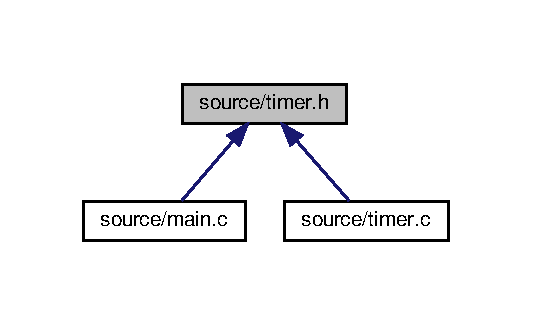
\includegraphics[width=256pt]{timer_8h__dep__incl}
\end{center}
\end{figure}
\subsection*{Functions}
\begin{DoxyCompactItemize}
\item 
void \hyperlink{timer_8h_a7fbd51d7ec681a9e21a3ae1cc242fc2e}{set\+\_\+timer\+\_\+duration} (int time\+\_\+in\+\_\+ms)
\begin{DoxyCompactList}\small\item\em Sets the duration of the timer. \end{DoxyCompactList}\item 
int \hyperlink{timer_8h_a227367655de202547cc62f7211cc5521}{start\+\_\+timer} (int($\ast$orders)\mbox{[}10\mbox{]}, int array\+\_\+size)
\begin{DoxyCompactList}\small\item\em Starts the timer and lets it run for the set timer duration unless the. obstruction button or stop button is pushed. \end{DoxyCompactList}\end{DoxyCompactItemize}


\subsection{Detailed Description}
Timer functionality. 



\subsection{Function Documentation}
\mbox{\Hypertarget{timer_8h_a7fbd51d7ec681a9e21a3ae1cc242fc2e}\label{timer_8h_a7fbd51d7ec681a9e21a3ae1cc242fc2e}} 
\index{timer.\+h@{timer.\+h}!set\+\_\+timer\+\_\+duration@{set\+\_\+timer\+\_\+duration}}
\index{set\+\_\+timer\+\_\+duration@{set\+\_\+timer\+\_\+duration}!timer.\+h@{timer.\+h}}
\subsubsection{\texorpdfstring{set\+\_\+timer\+\_\+duration()}{set\_timer\_duration()}}
{\footnotesize\ttfamily void set\+\_\+timer\+\_\+duration (\begin{DoxyParamCaption}\item[{int}]{time\+\_\+in\+\_\+ms }\end{DoxyParamCaption})}



Sets the duration of the timer. 


\begin{DoxyParams}{Parameters}
{\em time\+\_\+in\+\_\+ms} & Timer duration in milliseconds. \\
\hline
\end{DoxyParams}


Definition at line 12 of file timer.\+c.

\mbox{\Hypertarget{timer_8h_a227367655de202547cc62f7211cc5521}\label{timer_8h_a227367655de202547cc62f7211cc5521}} 
\index{timer.\+h@{timer.\+h}!start\+\_\+timer@{start\+\_\+timer}}
\index{start\+\_\+timer@{start\+\_\+timer}!timer.\+h@{timer.\+h}}
\subsubsection{\texorpdfstring{start\+\_\+timer()}{start\_timer()}}
{\footnotesize\ttfamily int start\+\_\+timer (\begin{DoxyParamCaption}\item[{int($\ast$)}]{orders\mbox{[}10\mbox{]},  }\item[{int}]{array\+\_\+size }\end{DoxyParamCaption})}



Starts the timer and lets it run for the set timer duration unless the. obstruction button or stop button is pushed. 


\begin{DoxyParams}{Parameters}
{\em orders} & Pointer to the queue. \\
\hline
{\em array\+\_\+size} & Size of the queue.\\
\hline
\end{DoxyParams}
\begin{DoxyReturn}{Returns}
1 if the obstruction button or stop button is pushed. 0 otherwise (after timer\+\_\+duration milliseconds). 
\end{DoxyReturn}


Definition at line 17 of file timer.\+c.


\hypertarget{utilities_8h}{}\section{source/utilities.h File Reference}
\label{utilities_8h}\index{source/utilities.\+h@{source/utilities.\+h}}


Various utilities to simplify interaction with hardware.  


This graph shows which files directly or indirectly include this file\+:
\nopagebreak
\begin{figure}[H]
\begin{center}
\leavevmode
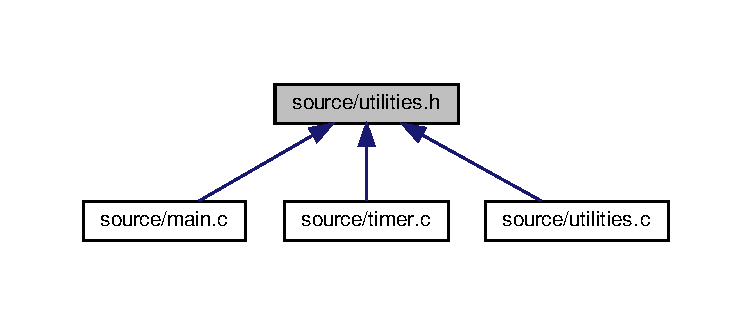
\includegraphics[width=350pt]{utilities_8h__dep__incl}
\end{center}
\end{figure}
\subsection*{Enumerations}
\begin{DoxyCompactItemize}
\item 
\mbox{\Hypertarget{utilities_8h_aa19be6305a5a4485e1e70de70ed7d677}\label{utilities_8h_aa19be6305a5a4485e1e70de70ed7d677}} 
enum \hyperlink{utilities_8h_aa19be6305a5a4485e1e70de70ed7d677}{states} \{ {\bfseries G\+O\+I\+N\+G\+\_\+\+UP}, 
{\bfseries I\+D\+LE}, 
{\bfseries G\+O\+I\+N\+G\+\_\+\+D\+O\+WN}, 
{\bfseries O\+R\+D\+E\+R\+\_\+\+E\+X\+P\+E\+D\+I\+T\+I\+ON}
 \}\begin{DoxyCompactList}\small\item\em State types used in the F\+SM in {\ttfamily main}. \end{DoxyCompactList}
\end{DoxyCompactItemize}
\subsection*{Functions}
\begin{DoxyCompactItemize}
\item 
int \hyperlink{utilities_8h_ab8de0eb632b04c75da60e750d632a752}{read\+\_\+current\+\_\+floor\+\_\+and\+\_\+set\+\_\+floor\+\_\+light} ()
\begin{DoxyCompactList}\small\item\em Checks if any of the floor sensors are active, and sets the corresponding floor light if it is. \end{DoxyCompactList}\item 
void \hyperlink{utilities_8h_a24f74ff4f31764f7b433abc4f4108534}{poll\+\_\+orders\+\_\+and\+\_\+add\+\_\+to\+\_\+queue} (int($\ast$orders)\mbox{[}10\mbox{]}, int array\+\_\+size)
\begin{DoxyCompactList}\small\item\em Polls order buttons and adds order to queue, {\ttfamily orders}, if button pressed. \end{DoxyCompactList}\item 
\mbox{\Hypertarget{utilities_8h_afd77151474c3e94d7c52fd75413ae3ca}\label{utilities_8h_afd77151474c3e94d7c52fd75413ae3ca}} 
void \hyperlink{utilities_8h_afd77151474c3e94d7c52fd75413ae3ca}{clear\+\_\+all\+\_\+order\+\_\+lights} ()
\begin{DoxyCompactList}\small\item\em Sets all order lights to 0 (off). \end{DoxyCompactList}\item 
\hyperlink{utilities_8h_aa19be6305a5a4485e1e70de70ed7d677}{states} \hyperlink{utilities_8h_ac7adbe2aa6f2118275091462f56ec972}{elevator\+\_\+init} ()
\begin{DoxyCompactList}\small\item\em Initializes elevator to a known state. \end{DoxyCompactList}\end{DoxyCompactItemize}


\subsection{Detailed Description}
Various utilities to simplify interaction with hardware. 



\subsection{Function Documentation}
\mbox{\Hypertarget{utilities_8h_ac7adbe2aa6f2118275091462f56ec972}\label{utilities_8h_ac7adbe2aa6f2118275091462f56ec972}} 
\index{utilities.\+h@{utilities.\+h}!elevator\+\_\+init@{elevator\+\_\+init}}
\index{elevator\+\_\+init@{elevator\+\_\+init}!utilities.\+h@{utilities.\+h}}
\subsubsection{\texorpdfstring{elevator\+\_\+init()}{elevator\_init()}}
{\footnotesize\ttfamily \hyperlink{utilities_8h_aa19be6305a5a4485e1e70de70ed7d677}{states} elevator\+\_\+init (\begin{DoxyParamCaption}{ }\end{DoxyParamCaption})}



Initializes elevator to a known state. 

\begin{DoxyReturn}{Returns}
Current state. 
\end{DoxyReturn}


Definition at line 38 of file utilities.\+c.

\mbox{\Hypertarget{utilities_8h_a24f74ff4f31764f7b433abc4f4108534}\label{utilities_8h_a24f74ff4f31764f7b433abc4f4108534}} 
\index{utilities.\+h@{utilities.\+h}!poll\+\_\+orders\+\_\+and\+\_\+add\+\_\+to\+\_\+queue@{poll\+\_\+orders\+\_\+and\+\_\+add\+\_\+to\+\_\+queue}}
\index{poll\+\_\+orders\+\_\+and\+\_\+add\+\_\+to\+\_\+queue@{poll\+\_\+orders\+\_\+and\+\_\+add\+\_\+to\+\_\+queue}!utilities.\+h@{utilities.\+h}}
\subsubsection{\texorpdfstring{poll\+\_\+orders\+\_\+and\+\_\+add\+\_\+to\+\_\+queue()}{poll\_orders\_and\_add\_to\_queue()}}
{\footnotesize\ttfamily void poll\+\_\+orders\+\_\+and\+\_\+add\+\_\+to\+\_\+queue (\begin{DoxyParamCaption}\item[{int($\ast$)}]{orders\mbox{[}10\mbox{]},  }\item[{int}]{array\+\_\+size }\end{DoxyParamCaption})}



Polls order buttons and adds order to queue, {\ttfamily orders}, if button pressed. 


\begin{DoxyParams}{Parameters}
{\em orders} & Pointer to queue. \\
\hline
{\em array\+\_\+size} & Size of queue array. \\
\hline
\end{DoxyParams}


Definition at line 18 of file utilities.\+c.

\mbox{\Hypertarget{utilities_8h_ab8de0eb632b04c75da60e750d632a752}\label{utilities_8h_ab8de0eb632b04c75da60e750d632a752}} 
\index{utilities.\+h@{utilities.\+h}!read\+\_\+current\+\_\+floor\+\_\+and\+\_\+set\+\_\+floor\+\_\+light@{read\+\_\+current\+\_\+floor\+\_\+and\+\_\+set\+\_\+floor\+\_\+light}}
\index{read\+\_\+current\+\_\+floor\+\_\+and\+\_\+set\+\_\+floor\+\_\+light@{read\+\_\+current\+\_\+floor\+\_\+and\+\_\+set\+\_\+floor\+\_\+light}!utilities.\+h@{utilities.\+h}}
\subsubsection{\texorpdfstring{read\+\_\+current\+\_\+floor\+\_\+and\+\_\+set\+\_\+floor\+\_\+light()}{read\_current\_floor\_and\_set\_floor\_light()}}
{\footnotesize\ttfamily int read\+\_\+current\+\_\+floor\+\_\+and\+\_\+set\+\_\+floor\+\_\+light (\begin{DoxyParamCaption}{ }\end{DoxyParamCaption})}



Checks if any of the floor sensors are active, and sets the corresponding floor light if it is. 

\begin{DoxyReturn}{Returns}
Floor number if floor sensor active. 0 otherwise. 
\end{DoxyReturn}


Definition at line 8 of file utilities.\+c.


%--- End generated contents ---

% Index
\backmatter
\newpage
\phantomsection
\clearemptydoublepage
\addcontentsline{toc}{chapter}{Index}
\printindex

\end{document}
